% !TeX root = ../../main_socg.tex

\begin{definition}[Surrounding Pair]
  Let $X$ be a topological space and $(D,B)$ a pair in $X$.
  The set $B$ \textbf{surrounds $D$ in $X$} if $B$ separates $X$ with the pair $(D\setminus B, X\setminus D)$.
  We will refer to such a pair as a \textbf{surrounding pair in $X$}.
\end{definition}

Let $(D, B)$ be a surrounding pair in $X$ and $U\subseteq D$, $V\subseteq U\cap B$ be subsets.
Let $\ell: \hom_0(X\setminus B, X\setminus D)\to \hom_0(X\setminus V, X\setminus U)$ be induced by inclusion.
The following lemma generalize the proof of the TCC as properties of surrounding sets, its proof can be found in the full version of this paper.

\begin{lemma}\label{lem:coverage}
  If $\ell$ is injective then $D\setminus B\subseteq U$ and $V$ surrounds $U$ in $D$.
\end{lemma}
\proofatend
  \begin{description}
    \item[$\ell$ injective $\implies$ $D\setminus B\subseteq U$] Suppose, for the sake of contradiction, that $p$ is injective and there exists a point $x\in (D\setminus B)\setminus U$.
      Because $B$ surrounds $D$ in $X$ the pair $(D\setminus B, \overline{D})$ forms a separation of $\overline{B}$.
      Therefore, $\hom_0(\overline{B})\cong \hom_0(D\setminus B)\oplus \hom_0(\overline{D})$ so
      \[ \hom_0(\overline{B}, \overline{D})\cong \hom_0(D\setminus B). \]
      So $[x]$ is non-trivial in $\hom_0(\overline{B},\overline{D})\cong \hom_0(D\setminus B)$ as $x$ is in some connected component of $D\setminus B$.
      So we have the following sequence of maps induced by inclusions
      \[ \hom_0(\overline{B},\overline{D})\xrightarrow{f} \hom_0(\overline{B},\overline{D}\cup\{x\})\xrightarrow{g} \hom_0(\overline{V},\overline{U}).\]
      As $f[x]$ is trivial in $\hom_0(\overline{B},\overline{D}\cup\{x\})$ we have that $\ell[x] = (g\circ f)[x]$ is trivial, contradicting our hypothesis that $\ell$ is injective.
    \item[$\ell$ injective $\implies$ $V$ surrounds $U$ in $D$.] Suppose, for the sake of contradiction, that $V$ does not surround $U$ in $D$.
      Then there exists a path $\gamma : [0,1]\to\overline{V}$ with $\gamma(0)\in U\setminus V$ and $\gamma(1)\in D\setminus U$.
      By Lemma~\ref{lem:coverage} we know that $D\setminus B\subseteq U$, so $D\setminus B\subseteq U\setminus V$.

      Choose $x\in D\setminus B$ and $z\in \overline{D}$ such that there exist paths $\xi : [0,1]\to U\setminus V$ with $\xi(0) = x$, $\xi(1) = \gamma(0)$ and $\zeta : [0,1]\to \overline{D}\cup (D\setminus U)$ with $\zeta(0) = z$, $\zeta(1) = \gamma(1)$.
      $\xi, \gamma$ and $\zeta$ all generate chains in $C_1(\overline{V}, \overline{U})$ and $\xi + \gamma + \zeta = \gamma^*\in C_1(\overline{V}, \overline{U})$ with $\partial\gamma^* = x + z$.
      Moreover, $z$ generates a chain in $C_0(\overline{U})$ as $\overline{D}\subseteq\overline{U}$.
      So $x = \partial\gamma^* + z$ is a relative boundary in $C_0(\overline{V}, \overline{U})$, thus $\ell[x] = \ell[z]$ in $\hom_0(\overline{V}, \overline{L})$.
      However, because $B$ surrounds $D$, $[x]\neq [y]$ in $\hom_0(\overline{B}, \overline{D})$ contradicting our assumption that $\ell$ is injective.
    \end{description}
\endproofatend

We now combine these results on the homology of surrounding pairs with information about both $\X$ as a metric space and our function.
Let $(\X,\dist)$ be a metric space and $D\subseteq \X$ be a compact subspace.
Let $f : D\to \R$ be a $c$-Lipschitz function and $B_\alpha = f^{-1}((-\infty, a])$ denote the $\alpha$-sublevel set of $f$ for $\alpha\in\R$.
We introduce a constant $\omega$ as a threshold that defines our ``boundary'' as a sub-levelset of the function $f$.
Let $P$ be a finite subset of $D$ and $Q_\alpha := P\cap B_\alpha$ for $\alpha\in\R$.
Let $\zeta\geq\delta > 0 $ and $\omega\in \R$ be constants such that $P^\delta\subseteq D$.
Here, $\delta$ will serve as our communication radius where $\zeta$ is reserved for use in Section~\ref{sec:middle}.
  \footnote{We will set $\zeta = 2\delta$ in the proof of our interleaving with Rips complexes but the TCC holds for all $\zeta\geq\delta$.}

\begin{lemma}\label{lem:psurj}
  Let $i : \hom_0(\cmp{\QQ^\of}, \cmp{P^\of})\to \hom_0(\cmp{\Q^\of}, \cmp{P^\delta})$.

  If $\B$ surrounds $D$ in $\X$ then $\dim~\hom_0(\cmp{\B}, \cmp{D})\geq \rk~i$.
\end{lemma}
\begin{proof}
  Choose a basis for $\im~i$ such that each basis element is represented by a point in $P^\of\setminus \QQ^\of$.
  Let $x\in P^\of\setminus \QQ^\of$ be such that $i[x] \neq 0$.
  So there exits some $p\in P$ such that $\dist(p, x) < \delta$ and $p\notin \QQ$, otherwise $x\in\QQ^\of$.
  Therefore, because $f$ is $c$-Lipschitz,
  \[ f(x)\geq f(p) - c\dist(x, p) > \fenn - c\of =\omega.\]

  So $x\in\cmp{\B}$ and, because $x\in P^\of\subseteq D$, $x\in D\setminus \B$.
  Because $i$ and $\ell : \hom_0(\cmp{\B}, \cmp{D})\to \hom_0(\cmp{\Q^\of}, \cmp{P^\of})$ are induced by inclusion $\ell[x] = i[x]\neq 0$ in $\hom_0(\cmp{\Q^\of}, \cmp{P^\of})$.
  That is, every element of $\im~i$ has a preimage in $\hom_0(\cmp{\B}, \cmp{D})$, so we may conclude that $\dim~\hom_0(\cmp{\B}, \cmp{D})\geq \rk~i$.
\end{proof}

Note that, while there is a surjective map from $\hom_0(\cmp{\B}, \cmp{D})$ to $\im~i$ this map is not necessarily induced by inclusion, as $\QQ^\of\not\subseteq \B$.
We therefore must introduce a larger space $B_{\omega+c(\delta+\zeta)}$ that contains $\QQ^\of$ in order to provide a criteria for the injectivity of $\ell : \hom_0(\cmp{\B}, \cmp{D})\to\hom_0(\cmp{\Q^\of}, \cmp{P^\of})$ in terms of $\rk~i$.

\[ \begin{tikzcd}
  (P^\of, \Q^\of) \arrow[hookrightarrow]{r}\arrow[hookrightarrow]{d} &
  (P^\of, \QQ^\of) \arrow[hookrightarrow]{d} \\
  %
  (D, \bb) \arrow[hookrightarrow]{r} &
  (D, B_{\omega+c(\delta+\zeta)}),
\end{tikzcd}\begin{tikzcd}
  (\cmp{B_{\omega+c(\delta+\zeta)}},\cmp{D})\arrow[hookrightarrow]{d}\arrow[hookrightarrow]{r} &
  (\cmp{\bb}, \cmp{D}) \arrow[hookrightarrow]{d}\\
  %
  (\cmp{\QQ^\of}, \cmp{P^\of}) \arrow[hookrightarrow]{r} &
  (\cmp{\Q^\of}, \cmp{P^\of}).
\end{tikzcd}\]

\begin{equation}\label{dgm:1}\begin{tikzcd}
  \hom_0(\cmp{B_{\omega+c(\delta+\zeta)}},\cmp{D})\arrow{d}{m} \arrow{r}{j} &
  \hom_0(\cmp{\bb}, \cmp{D}) \arrow{d}{\ell} \\
  %
  \hom_0(\cmp{\QQ^\of}, \cmp{P^\of}) \arrow{r}{i} &
  \hom_0(\cmp{\Q^\of}, \cmp{P^\of}).
\end{tikzcd}\end{equation}

\paragraph{Assumptions}

We will first require the map $\hom_0(D\setminus B_{\omega+c(\delta+\zeta)}\hookrightarrow D\setminus B_\omega)$ to be \emph{surjective}---as we approach $\omega$ from \emph{above} no components \emph{appear}.
This ensures that the rank of the map $j$ is equal to the dimension of $\dim~\hom_0(\cmp{B_\omega}, \cmp{D})$ so our map $\ell$ induced by inclusion depends only on $\hom_0(\cmp{B_\omega}, \cmp{D})$ and $\im~i$.
% That is, in terms of $\omega$ as a super-levelset monotonically decreasing, no components \emph{apear} right \emph{before} $\omega$.
% We note that, for a function in two dimensions, this translates to $1$-dimensional features disappearing right after $\omega$ in the sub-levelset filtration, as shown in Figure~\ref{fig:assumption1}.

\begin{figure}[htbp]\label{fig:assumption1}
  \centering
  
\includegraphics[trim=200 300 200 200, clip, width=0.5\textwidth]{scripts/figures/surf/ass1_C_side.png}
  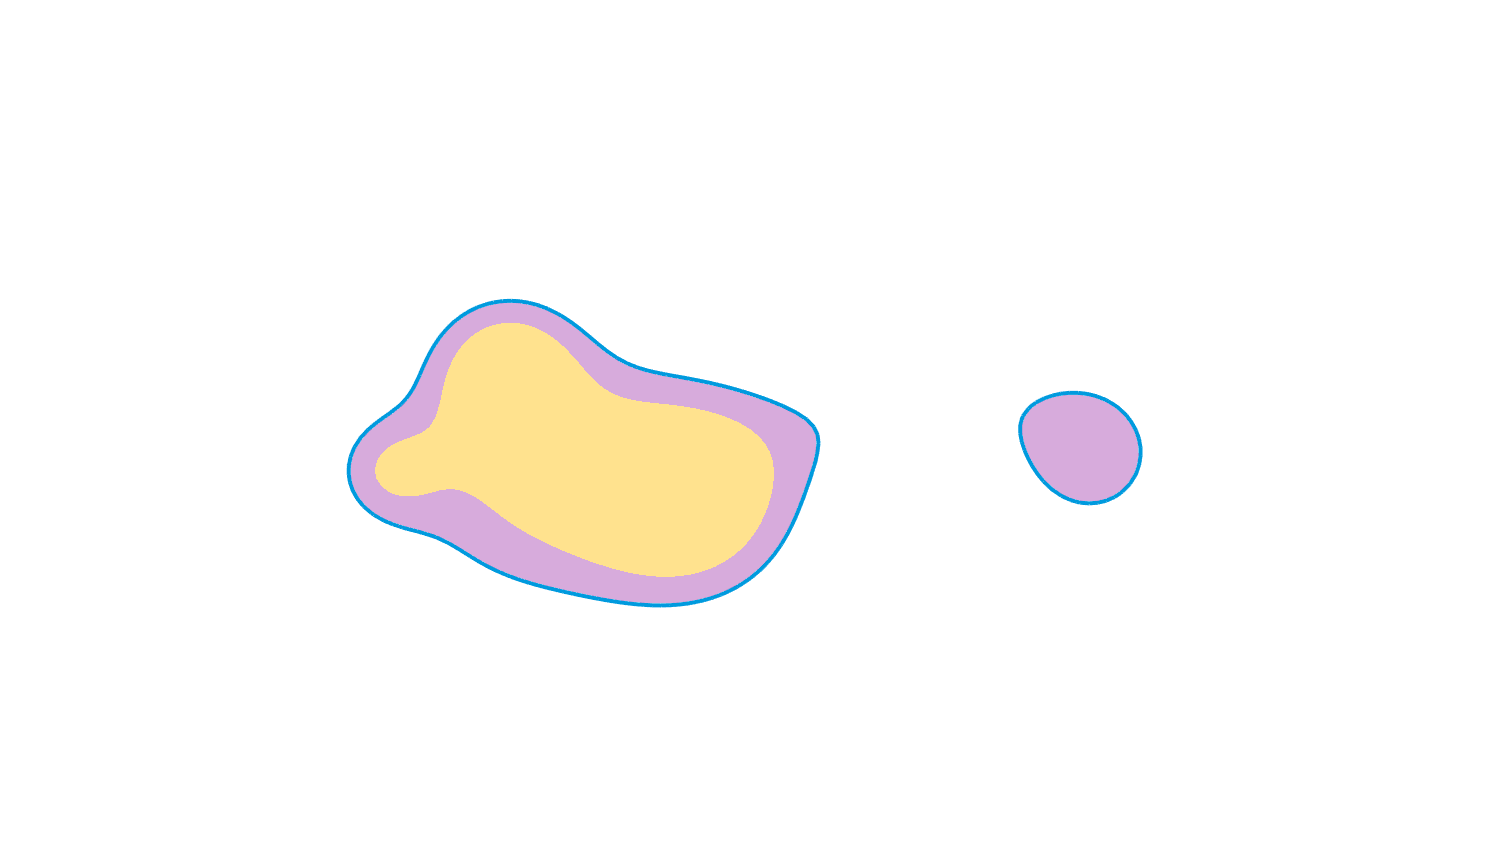
\includegraphics[trim=300 150 200 200, clip, width=0.3\textwidth]{scripts/figures/surf/ass1_C_top.png}
  
\includegraphics[trim=200 300 200 200, clip, width=0.5\textwidth]{scripts/figures/surf/ass1_D_side.png}
  
\includegraphics[trim=300 150 200 200, clip, width=0.3\textwidth]{scripts/figures/surf/ass1_D_top.png}
  
\includegraphics[scale=0.7]{scripts/figures/scalar_barcode_H1-masked.png}
  \caption{\textbf{(Assumption 1)} The blue levelset does not satisfy Assumption 1 as the smaller component is ``pinched out'' in the orange region.}
            % This can be seen in the barcode shown as a feature that dies in the purple region.}
\end{figure}

We also assume that $\hom_0(D\setminus B_\omega\hookrightarrow D\setminus B_{\omega-c(\delta+\zeta)})$ is \emph{injective}---as we move away from $\omega$ moving \emph{down} no components \emph{disappear}.
Lemma~\ref{lem:assumption2} uses Assumption 2 to provide a computable upper bound on $\rk~j$, its proof can be found in the full version of this paper.
% Once again, in terms of $\omega$ as a superlevel set monotonically decreasing, no components \emph{disappear} right \emph{after} $\omega$.
% Once again, for a function in two dimensions, this translates to features in dimension 1 appearing before $\omega$ is the sublevel set filtration, as shown in Figure~\ref{fig:assumption2}.

\begin{figure}[htbp]\label{fig:assumption2}
  \centering
  
\includegraphics[trim=200 300 200 200, clip, width=0.5\textwidth]{scripts/figures/surf/ass2_C_side.png}
  
\includegraphics[trim=300 200 200 200, clip, width=0.3\textwidth]{scripts/figures/surf/ass2_C_top.png}
  
\includegraphics[trim=200 300 200 200, clip, width=0.5\textwidth]{scripts/figures/surf/ass2_B_side.png}
  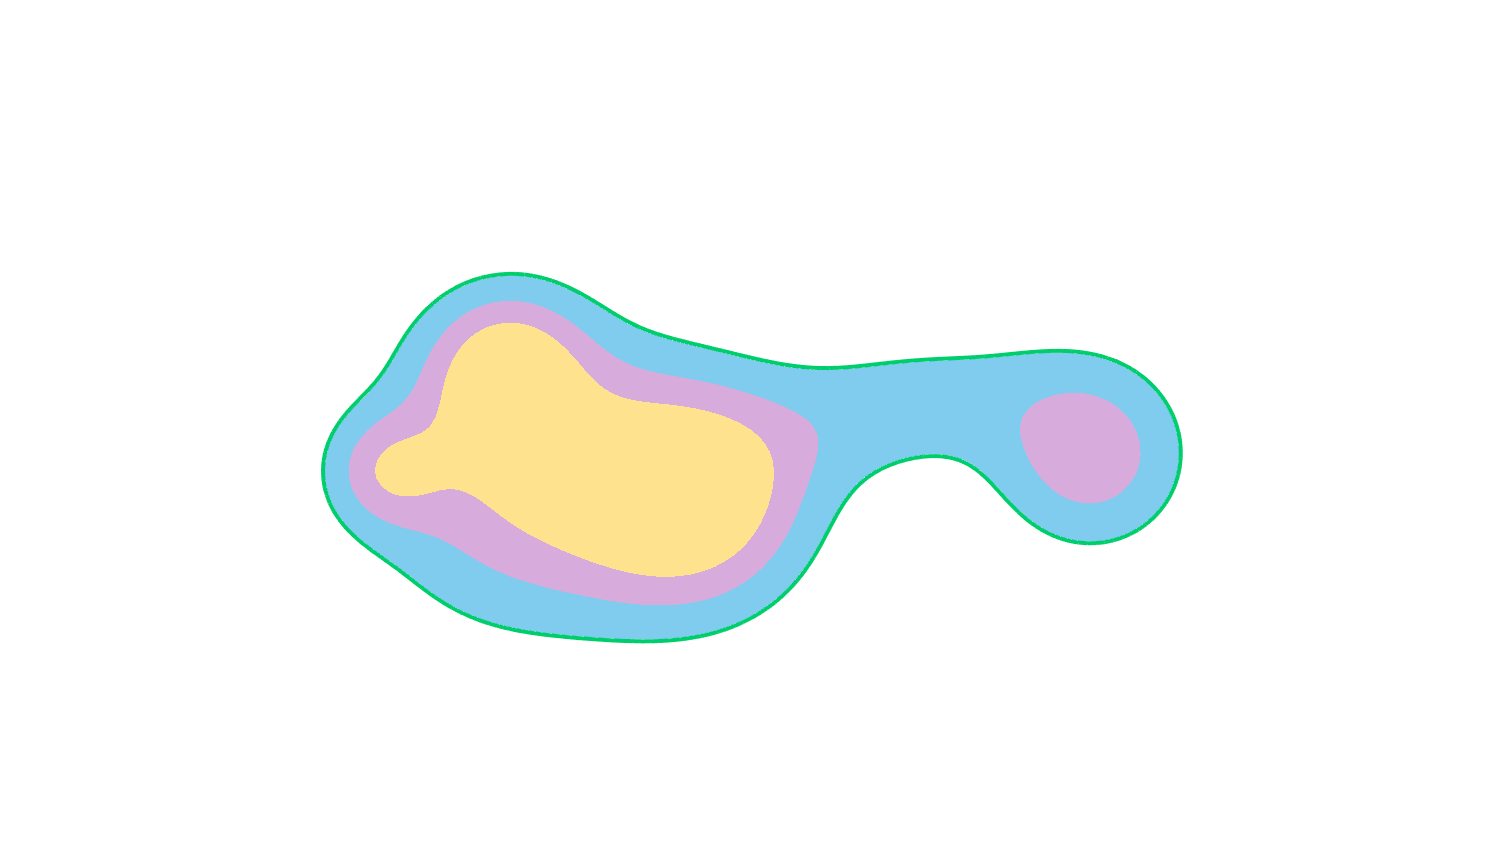
\includegraphics[trim=300 200 200 200, clip, width=0.3\textwidth]{scripts/figures/surf/ass2_B_top.png}
  
\includegraphics[scale=0.7]{scripts/figures/scalar_barcode_H1-masked.png}
  \caption{\textbf{(Assumption 2)} The blue levelset does not satisfy Assumption 2 as the smaller component is not in the inclusion from blue to green.}
          % This can be seen in the second feature of the barcode shown as a feature which is born in the blue region.}
\end{figure}

\begin{lemma}\label{lem:assumption2}
  If $\hom_0(D\setminus B_\omega\hookrightarrow D\setminus B_{\omega+c(\delta+\zeta)})$ is injective and each component of $D\setminus B_\omega$ contains a point in $P$ then $\dim~\hom_0(\rips^\delta(P\setminus Q_{\omega-c\zeta})) \geq \dim~\hom_0(D\setminus B_\omega)$.
\end{lemma}
\proofatend
  Assume there exist $p,q \in P\setminus Q_{\omega-c\zeta}$ such that $p$ and $q$ are connected in $\rips^\delta(P\setminus Q_{\omega-c\zeta})$ but not in $D\setminus B_\omega$.
  So the shortest path from $p, q$ is a subset of $(P\setminus Q_{\omega-c\zeta})^\delta$.
  For any $x\in (P\setminus Q_{\omega-c\zeta})^\delta$ there exists some $p\in P$ such that $f(p) > \omega - c\zeta$ and $\dist(p,x) < \delta$.
  Because $f$ is $c$-Lipschitz
  \[ f(x)\geq f(p) - c\dist(x,p) > \omega - c(\delta+\zeta)\]
  so there is a path from $p$ to $q$ in $D\setminus B_{\omega-c(\delta+\zeta)}$, thus $[p] = [q]$ in $\hom_0(D\setminus B_{\omega-c(\delta+\zeta)})$.

  But we have assumed that $[p]\neq[q]$ in $\hom_0(D\setminus B_\omega)$, contradicting our assumption that $\hom_0(D\setminus B_\omega\hookrightarrow D\setminus B_{\omega-c(\delta+\zeta)})$ is injective, so any $p,q$ connected in $\rips^\delta(P\setminus Q_{\omega-c\zeta})$ are connected in $D\setminus B_\omega$.
  That is, $\dim~\hom_0(\rips^\delta(P\setminus Q_{\omega-c\zeta}))\geq \dim~\hom_0(D\setminus B_\omega)$.
\endproofatend

% The statement of Theorem~\ref{thm:geo_tcc} is in terms of the $0$-dimensional homology of complement spaces makes it difficult, if not impossible, to compute directly.
% The following lemma
The full version of this paper details how to construct the following isomorphism using the Nerve Theorem along with Alexander Duality and the Universal Coefficient Theorem.
\[ \xi\N_w^{\e,k} : \hom_d(\cech^\e(P,Q_w))\to \hom_0(D\setminus Q_w^\e, D\setminus P^\e).\]
This isomorphism holds in the specific case when $P^\e\subseteq \intr_\X(D)$ and $D\setminus P^\e$, $D\setminus Q_w^\e$ are locally contractible.
We therefore provide the following definition for ease of exposition
\begin{definition}[$(\delta,\zeta,\omega)$-Sublevel Sample]
  For $\zeta\geq \delta > 0$, $\omega\in\R$, and a $c$-Lipschitz function $f: D\to \R$ a finite point set $P\subset D$ is said to be a \textbf{$(\delta, \zeta, \omega)$-sublevel sample} of $f$ if every component of $D\setminus B_\omega$ contains a point in $P$, $P^\delta\subset\intr_\X(D)$, and $D\setminus P^\delta$, $D\setminus Q_{\omega-c\zeta}^\delta$, and $D\setminus Q_{\omega+c\delta}^\delta$ are locally path connected in $\X$.
\end{definition}

\begin{theorem}[Algorithmic TCC]\label{thm:algo_tcc}
  Let $\X$ be an orientable $d$-manifold and let $D$ be a compact subset of $\X$.
  Let $f : D\to\R$ be $c$-Lipschitz function and $\omega\in\R$ and $\delta\leq\zeta < \varrho_D$ be constants such that $P\subset D$ is a $(\delta,\zeta,\omega)$-sublevel sample of $f$ and $B_{\omega - c(\zeta +\delta)}$ surrounds $D$ in $\X$.

  If $\hom_0(D\setminus B_{\omega+c(\delta+\zeta)}\hookrightarrow D\setminus B_\omega)$ is surjective, $\hom_0(D\setminus B_\omega\hookrightarrow D\setminus B_{\omega+c(\delta+\zeta)})$ is injective, and
  \[\rk~\hom_d(\rips^\delta(P, Q_{\omega -c\zeta})\hookrightarrow \rips^{2\delta}(P, Q_{\omega+c\delta})) \geq \dim~\hom_0(\rips^\delta(P\setminus Q_{\omega-c\zeta}))\]
  then $D\setminus B_\omega\subseteq P^\delta$ and $Q_{\omega-c\zeta}^\delta$ surrounds $P^\delta$ in $D$.
\end{theorem}
\begin{proof}
  % We have the following commutative diagram
  % \[\begin{tikzcd}
  %   \hom_d(\cech^\delta(P, Q_{\omega-c\zeta})) \arrow{r}{q_{\cech}}\arrow{d}{\N_{\omega-c\zeta}^{\delta}} &
  %   \hom_d(\cech^\delta(P, Q_{\omega+c\delta})) \arrow{d}{\N_{\omega-c\zeta}^\delta}\\
  %   %
  %   \hom_d(P^\delta, Q_{\omega-c\zeta}^\delta))\arrow{r}{q} &
  %   \hom_d(P^\delta, Q_{\omega+c\delta}^\delta).
  % \end{tikzcd}\]
  % where vertical maps are isomorphisms provided by the Nerve Theorem and horizontal maps are induced by inclusions.

  Because $P$ is a $(\delta, \zeta, \omega)$-sublevel sample we have isomorphisms $\xi\N_{\omega-c\zeta}^\delta$ and $\xi\N_{\omega+c\delta}^\delta$ that commute with $q_{\cech}$ and $i : \hom_0(D\setminus Q_{\omega+c\delta}^\delta, D\setminus P^\delta)\to \hom_0(D\setminus Q_{\omega-c\zeta}^\delta, D\setminus P^\delta)$.
  Let $q_{\rips} : \hom_d(\rips^{\delta}(P, Q_{\omega-c\zeta}))\to\hom_d(\rips^{2\delta}(P, Q_{\omega+c\delta}))$ be induced by inclusion.
  Then $\rk~q_{\cech} \geq\rk~q_{\rips}$ as $q_{\rips}$ factors through $q_{\cech}$.
  As we have assumed $\hom_0(D\setminus B_\omega\hookrightarrow D\setminus B_{\omega-c(\delta+\zeta)})$ Lemma~\ref{lem:assumption2} implies $\dim~\hom_0(\rips^\delta(P\setminus Q_{\omega-c\zeta}))\geq \dim~\hom_0(D\setminus B_\omega)$.
  It follows that, whenever $\rk~q_{\rips} \geq \dim~\hom_0(\rips^\delta(P\setminus Q_{\omega-c\zeta}))$, we have
  \[ \rk~i = \rk~q_{\cech} \geq \rk~q_{\rips} \geq \dim~\hom_0(\rips^\delta(P\setminus Q_{\omega-c\zeta})) \geq \dim~\hom_0(D\setminus B_\omega).\]

  Because $j$ is surjective by hypothesis $\rk~j = \dim~\hom_0(\cmp{\B},\cmp{D}) = \dim~\hom_0(D\setminus B_\omega)$ so $\rk~j\geq \rk~i$ by Lemma~\ref{lem:psurj}.
  Therefore, $\rk~j = \rk~i$ as we have shown $\rk~i\geq \dim~\hom_0(D\setminus B_\omega)$.
  Because $P$ is a finite point set we know that $\im~i$ is finite-dimensional and, because $\rk~i = \rk~j$, $\im~j=\hom_0(\cmp{\B}, \cmp{D})$ is finite dimensional as well.
  So $\im~j$ is isomorphic to $\im~i$ as a subspace of $\hom_0(\cmp{\Q^\of}, \cmp{P^\of})$ which, because $j$ is surjective, requires the map $\ell$ induced by inclusion to be injective.
  Therefore $D\setminus\bb\subseteq P^\of$ and $\Q^\of$ surrounds $P^\of$ in $D$ by Lemma~\ref{lem:coverage}.
  %, Lemma~\ref{lem:cov_surrounds}.
  % As $j : \hom_0(D\setminus B_{\omega+c(\delta+\zeta)})\to \hom_0(D\setminus B_\omega)$ is surjective by assumption $\rk~j = \dim~\hom_0(D\setminus B_\omega)$, so $D\setminus B_\omega\subseteq P^\delta$ and $Q_{\omega-c\zeta}^\delta$ surrounds $P^\delta$ in $D$ by Theorem~\ref{thm:geo_tcc} as desired.
\end{proof}
